\documentclass[17pt]{beamer} %Makes presentation
%\documentclass[handout, 17pt]{beamer} %Makes Handouts
\documentclass[14pt]{beamer} %Makes presentation
%\documentclass[handout]{beamer} %Makes Handouts
\usetheme{Singapore} %Gray with fade at top
\useoutertheme[subsection=false]{miniframes} %Supppress subsection in header
\useinnertheme{rectangles} %Itemize/Enumerate boxes
\usecolortheme{seagull} %Color theme
\usecolortheme{rose} %Inner color theme

\definecolor{light-gray}{gray}{0.75}
\definecolor{dark-gray}{gray}{0.55}
\setbeamercolor{item}{fg=light-gray}
\setbeamercolor{enumerate item}{fg=dark-gray}

\setbeamertemplate{navigation symbols}{}
%\setbeamertemplate{mini frames}[default]
\setbeamercovered{dynamics}
\setbeamerfont*{title}{size=\Large,series=\bfseries}

%\setbeameroption{notes on second screen} %Dual-Screen Notes
%\setbeameroption{show only notes} %Notes Output

\setbeamertemplate{frametitle}{\vspace{.5em}\bfseries\insertframetitle}
\newcommand{\heading}[1]{\noindent \textbf{#1}\\ \vspace{1em}}

\usepackage{bbding,color,multirow,times,ccaption,tabularx,graphicx,verbatim,booktabs,fixltx2e}
\usepackage{colortbl} %Table overlays
\usepackage[english]{babel}
\usepackage[latin1]{inputenc}
\usepackage[T1]{fontenc}
\usepackage{lmodern}

%\author[]{Thomas J. Leeper}
\institute[]{
  \inst{}%
  Department of Government\\London School of Economics and Political Science
}

\usepackage{tikz}
\usetikzlibrary{shapes,arrows,decorations.pathreplacing,calc}

\newcounter{itemnum}

\newcommand{\nt}[2][0pt]{%
    \stepcounter{itemnum}%
    \if###2##%
    \else
        #2%
        \thinspace
    \fi
    \tikz[overlay,remember picture,baseline=(\theitemnum.base),xshift=#1]\node (\theitemnum){};%
}

\newcommand{\makebrace}[4][0pt]{%
    \begin{tikzpicture}[overlay, remember picture]
        \draw [decoration={brace,amplitude=0.5em},decorate]
        let \p1=(#2), \p2=(#3) in
        ({max(\x1+#1,\x2+#1)}, {\y1+1.75ex}) -- 
            node[right=0.6em] {#4} ({max(\x1+#1,\x2+#1)}, {\y2-0.5ex});
    \end{tikzpicture}%
}

\newenvironment{braceitems}{%
    \begin{enumerate}
}{%
    \end{enumerate}
    \setcounter{itemnum}{0}%
}


\title{Measurement:\\Concepts in Practice}

% To study something, we need to be able to observe and measure it. How do we \textit{operationalize} concepts so that we can study political phenomena? What are challenges of measuring concepts? How do we assign quantitative values to observations?

\date[]{}

\begin{document}

\frame{\titlepage}

\frame{\tableofcontents}


\section{Observation and Description}
\frame{\tableofcontents[currentsection]}


\frame{

\frametitle{{\large Goals of Descriptive Research}}

\begin{enumerate}\itemsep1em
\item To \textit{answer} research questions
\item To \textit{generate} research questions
\item<2-> To do both of these, \textit{iteratively}
\end{enumerate}

}


\frame{

\frametitle{{\normalsize Ex.: Galileo's Drawings of Sunspots}}

\vspace{1em}

\href{http://galileo.rice.edu/sci/observations/ssm_slow.mpg}{\includegraphics[width=\textwidth]{images/sunspotspanel.png}}

\vspace{2em}

{\tiny
Source: Public Domain, \href{http://earthobservatory.nasa.gov/Features/SolarMax/}{NASA}
}
}



\frame{

\frametitle{{\normalsize Ex.: Broad Street Cholera}}

\begin{itemize}\itemsep0.5em
\item 1854 outbreak of cholera in London
	\begin{itemize}
	\item Around Broad Street (Soho)
	\item 616 eventual deaths
	\end{itemize}
\item<2-> Causal RQ: What causes transmission of cholera?
\item<3-> Descriptive RQ: Who exactly is contracting cholera?
\end{itemize}

}

\frame{
\begin{center}
\only<1>{\includegraphics[height=.98\textheight]{images/broadstreet}}
\only<2>{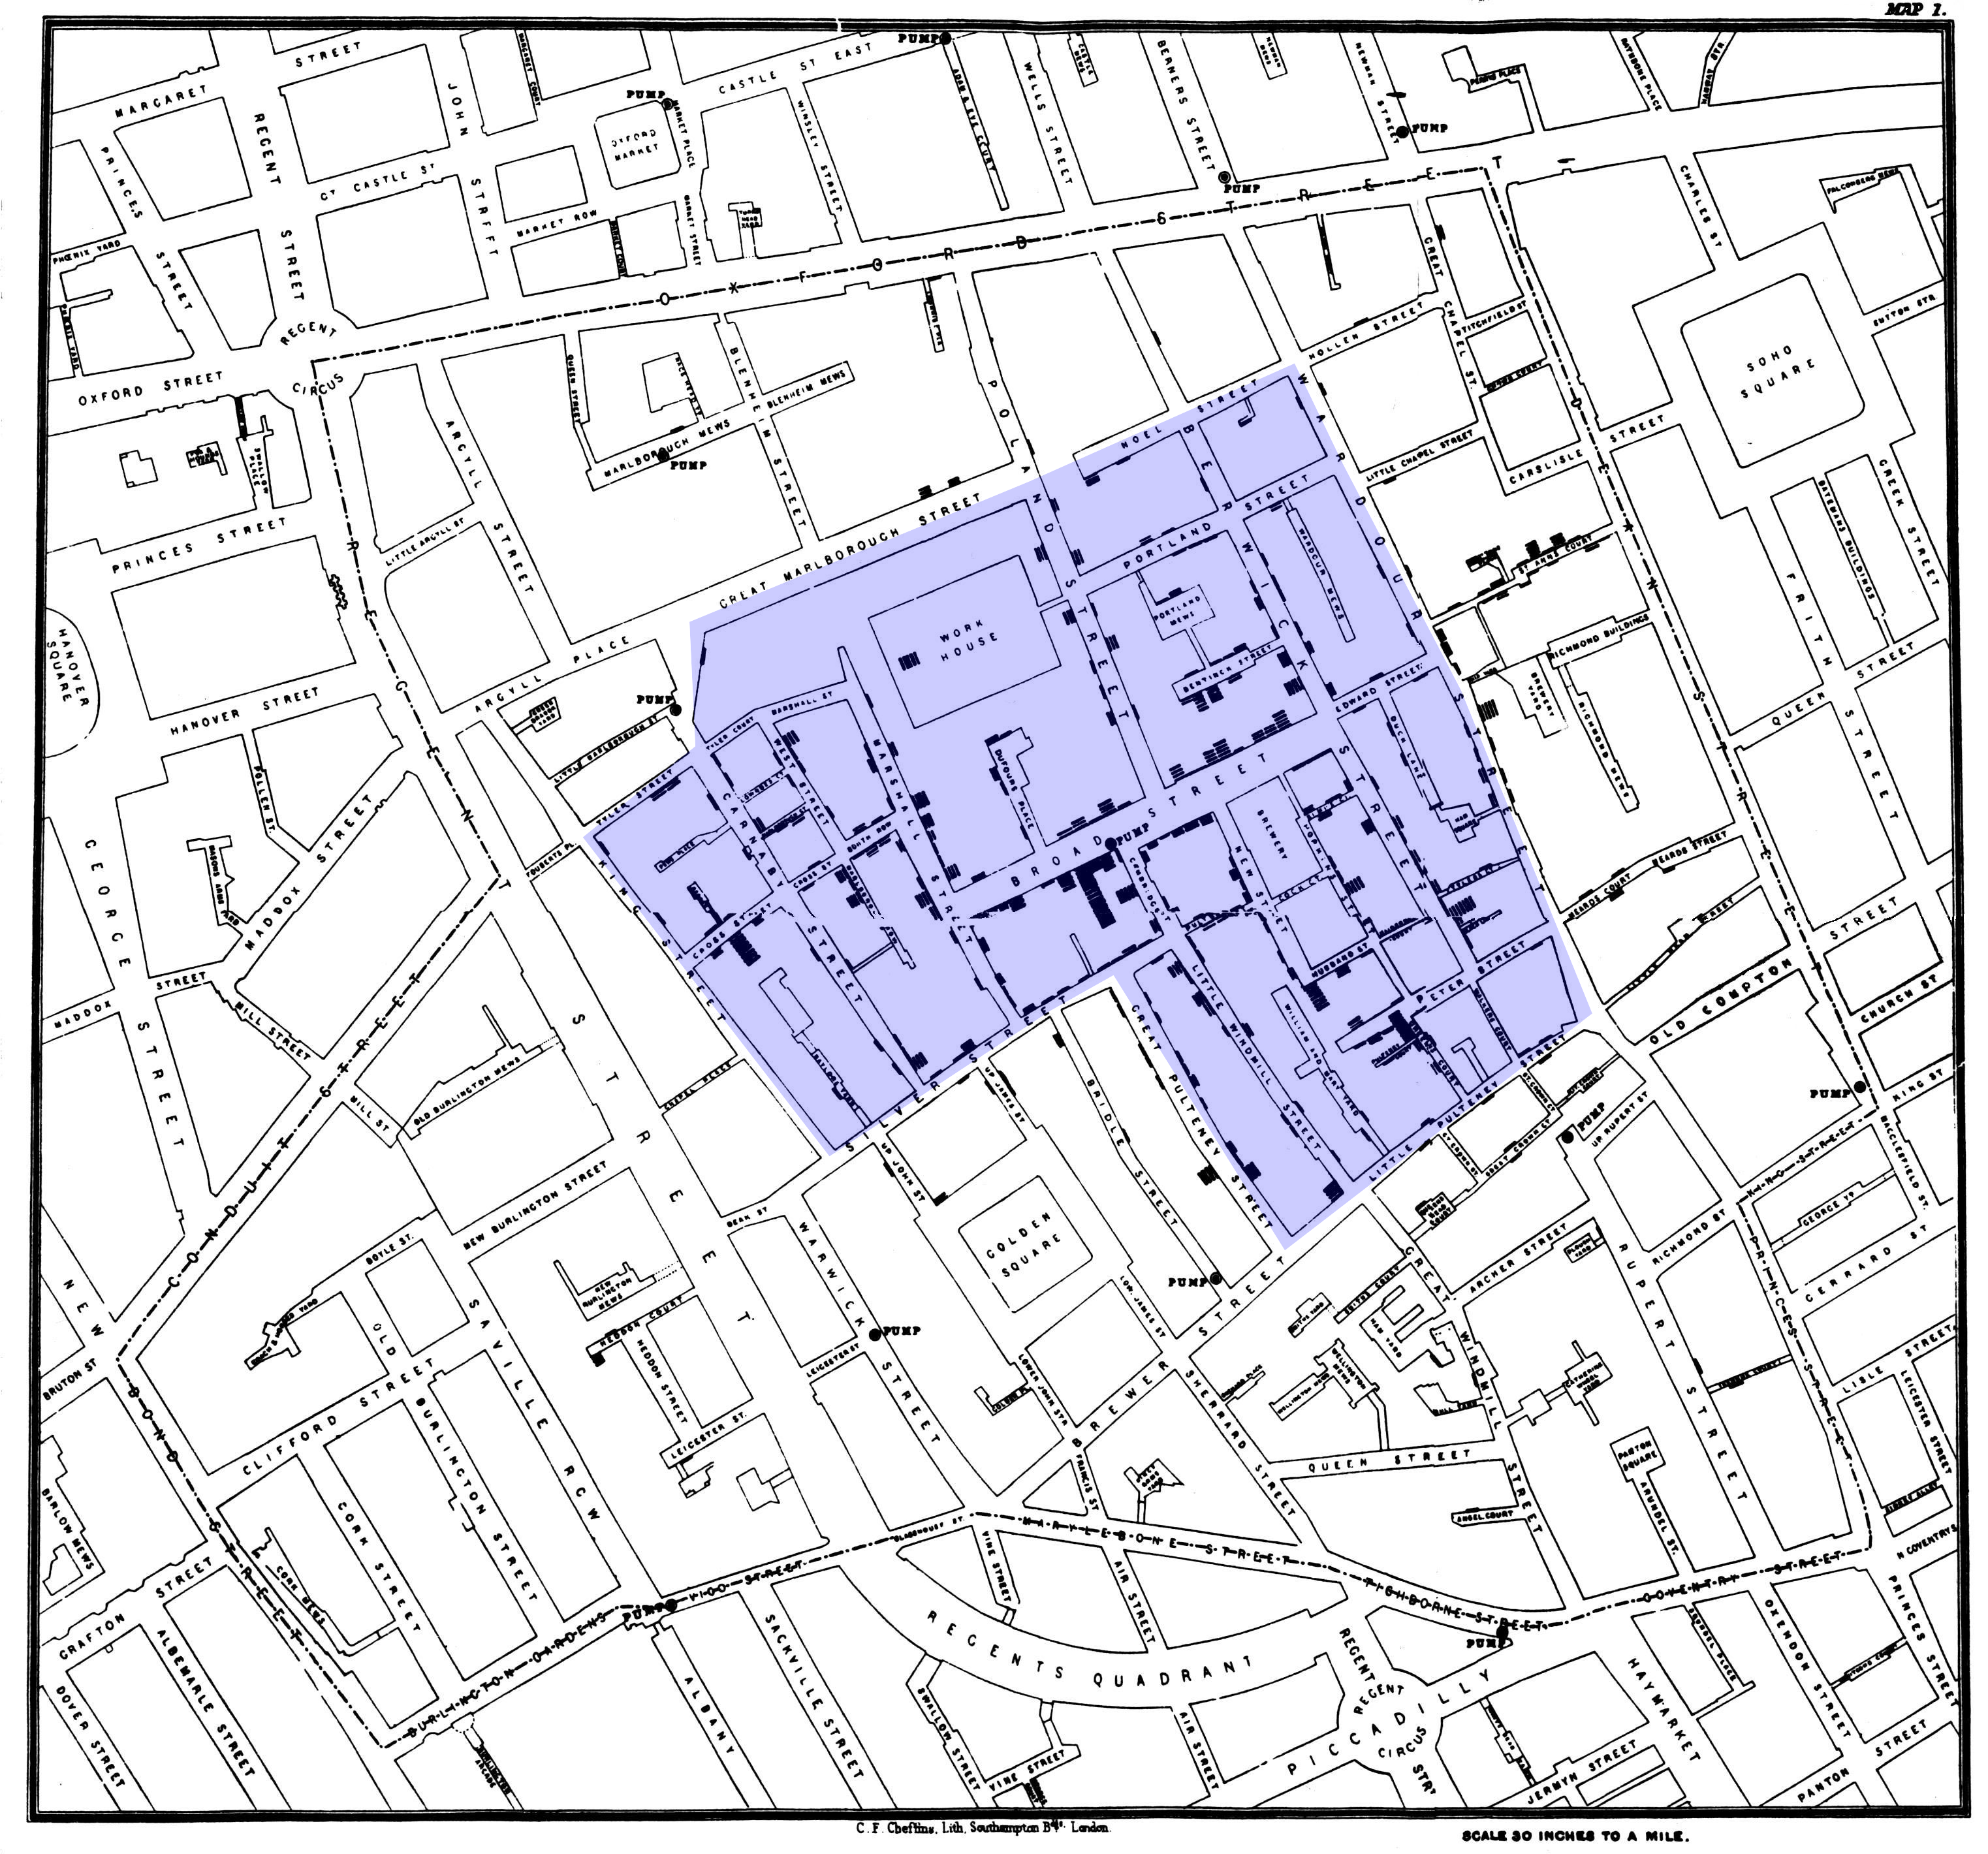
\includegraphics[height=.98\textheight]{images/broadstreet-1}}
\only<3>{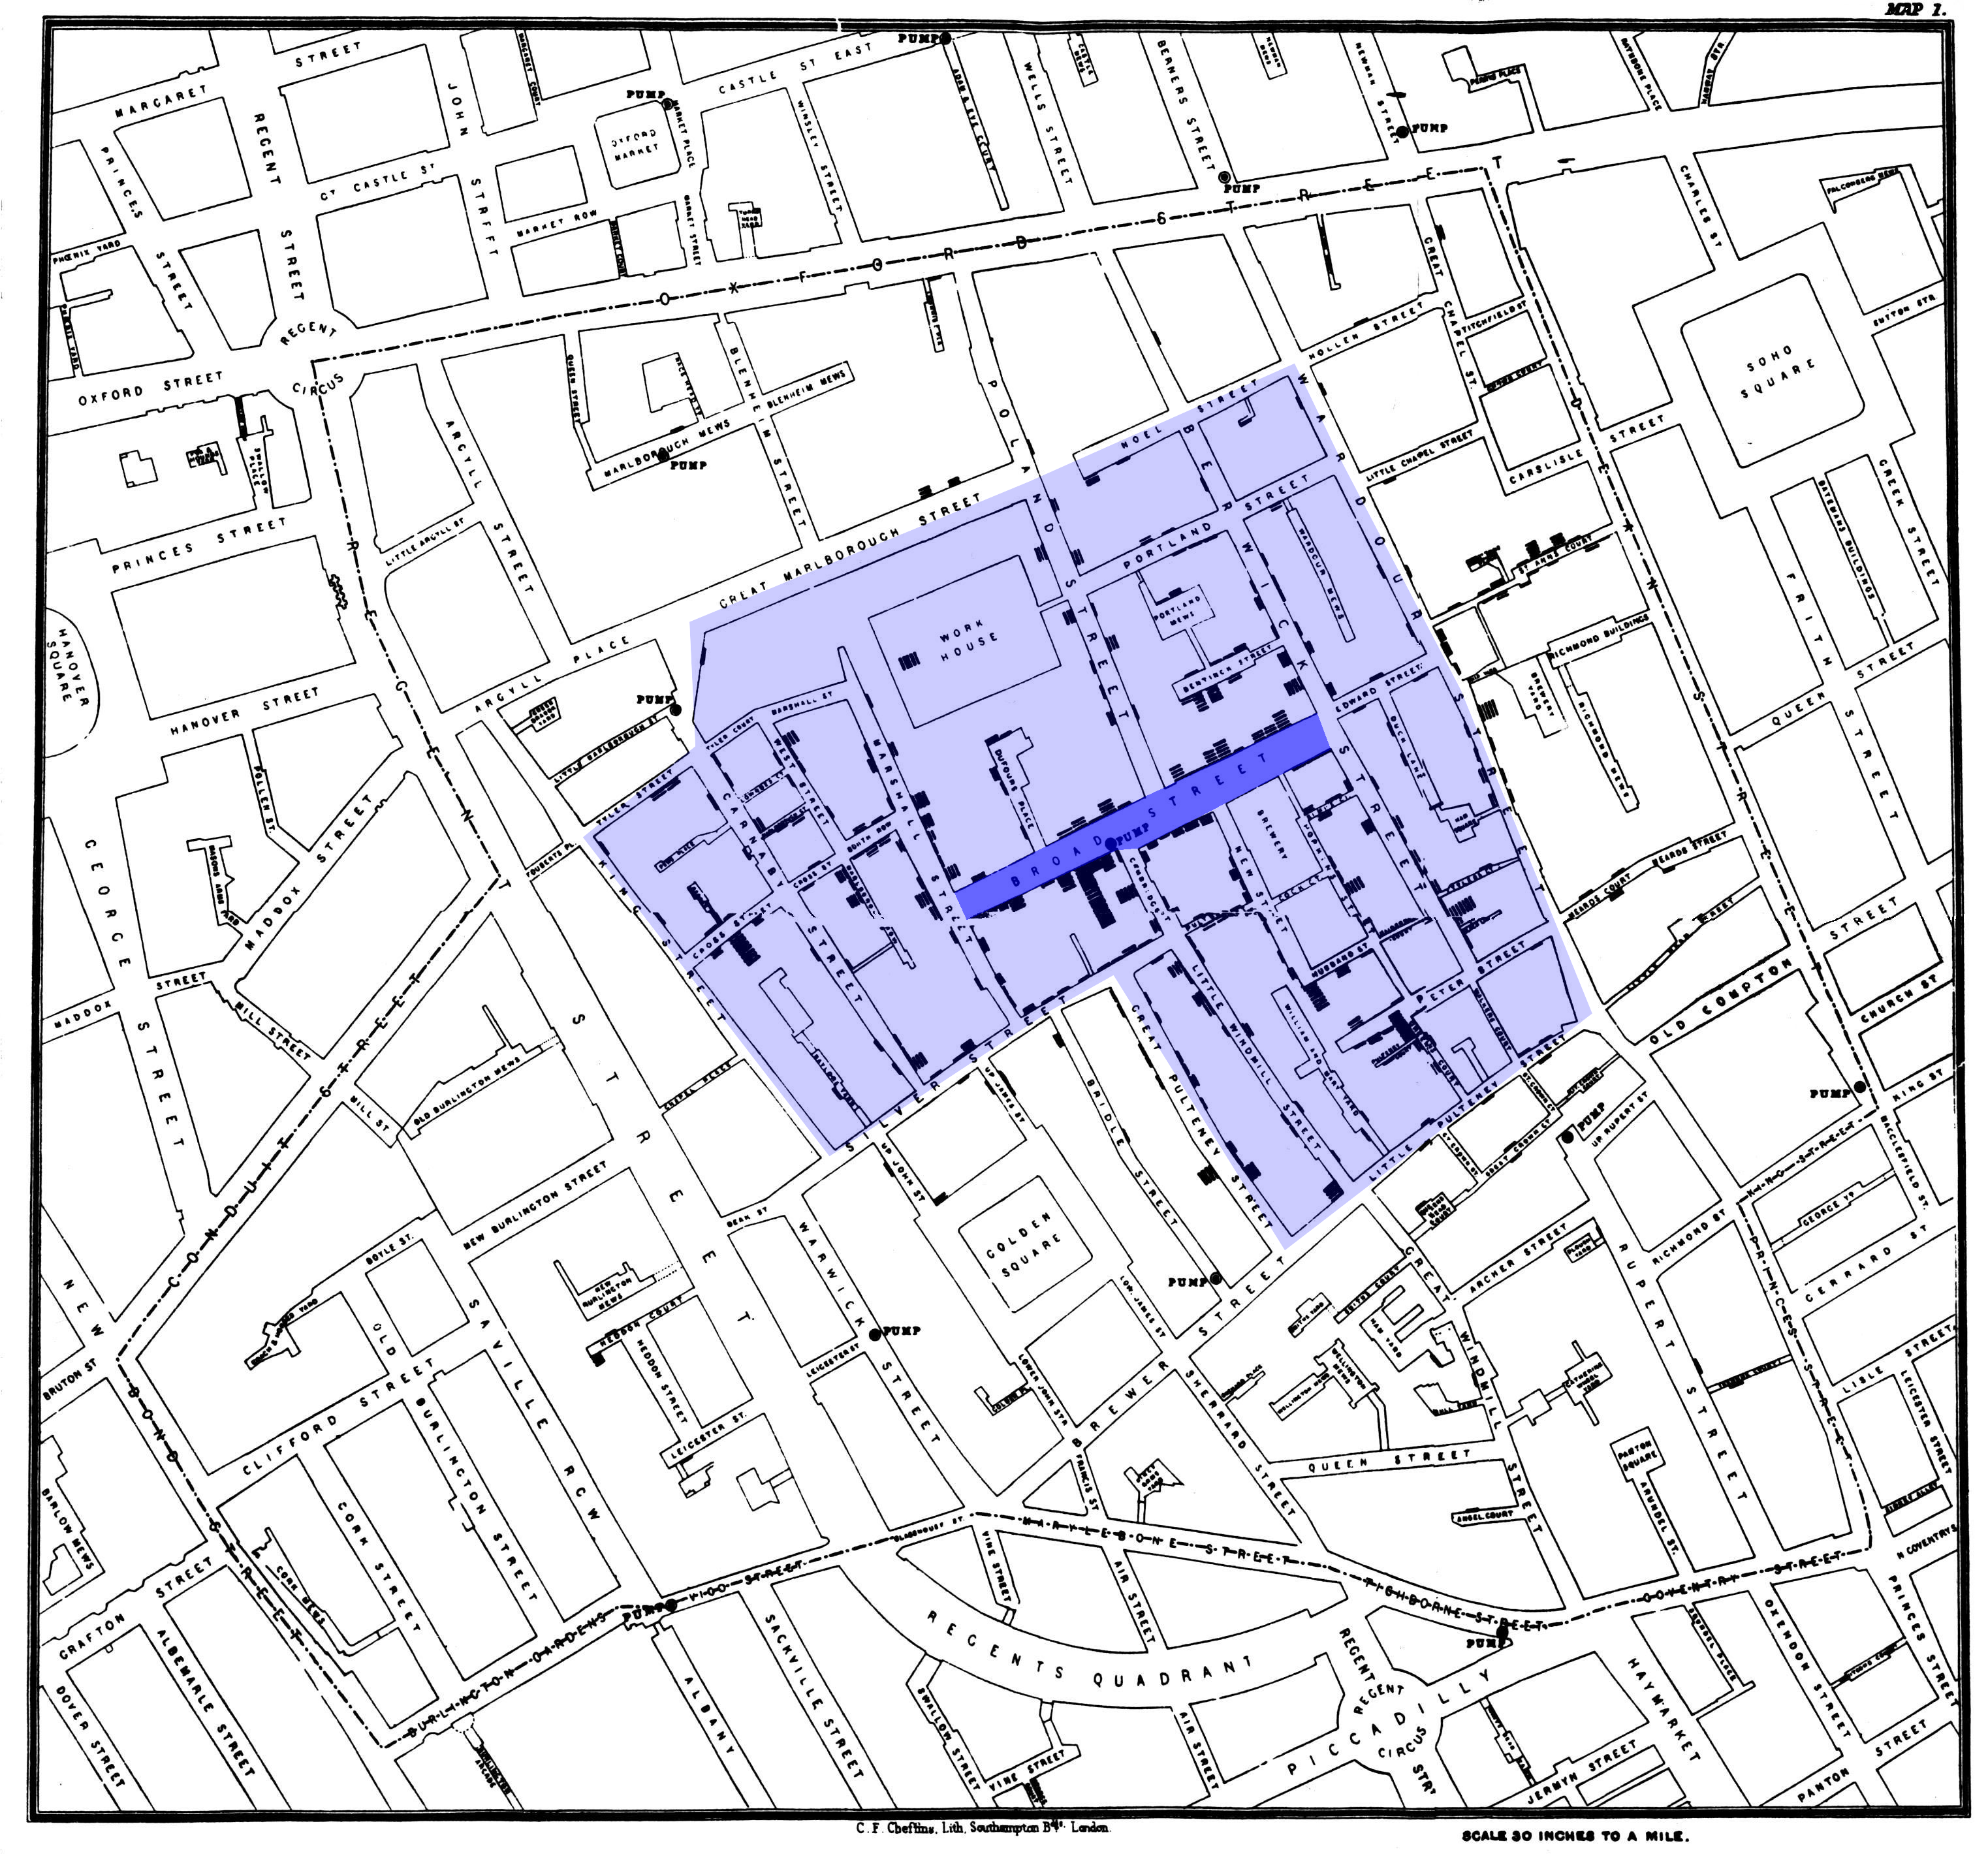
\includegraphics[height=.98\textheight]{images/broadstreet-2}}
\only<4>{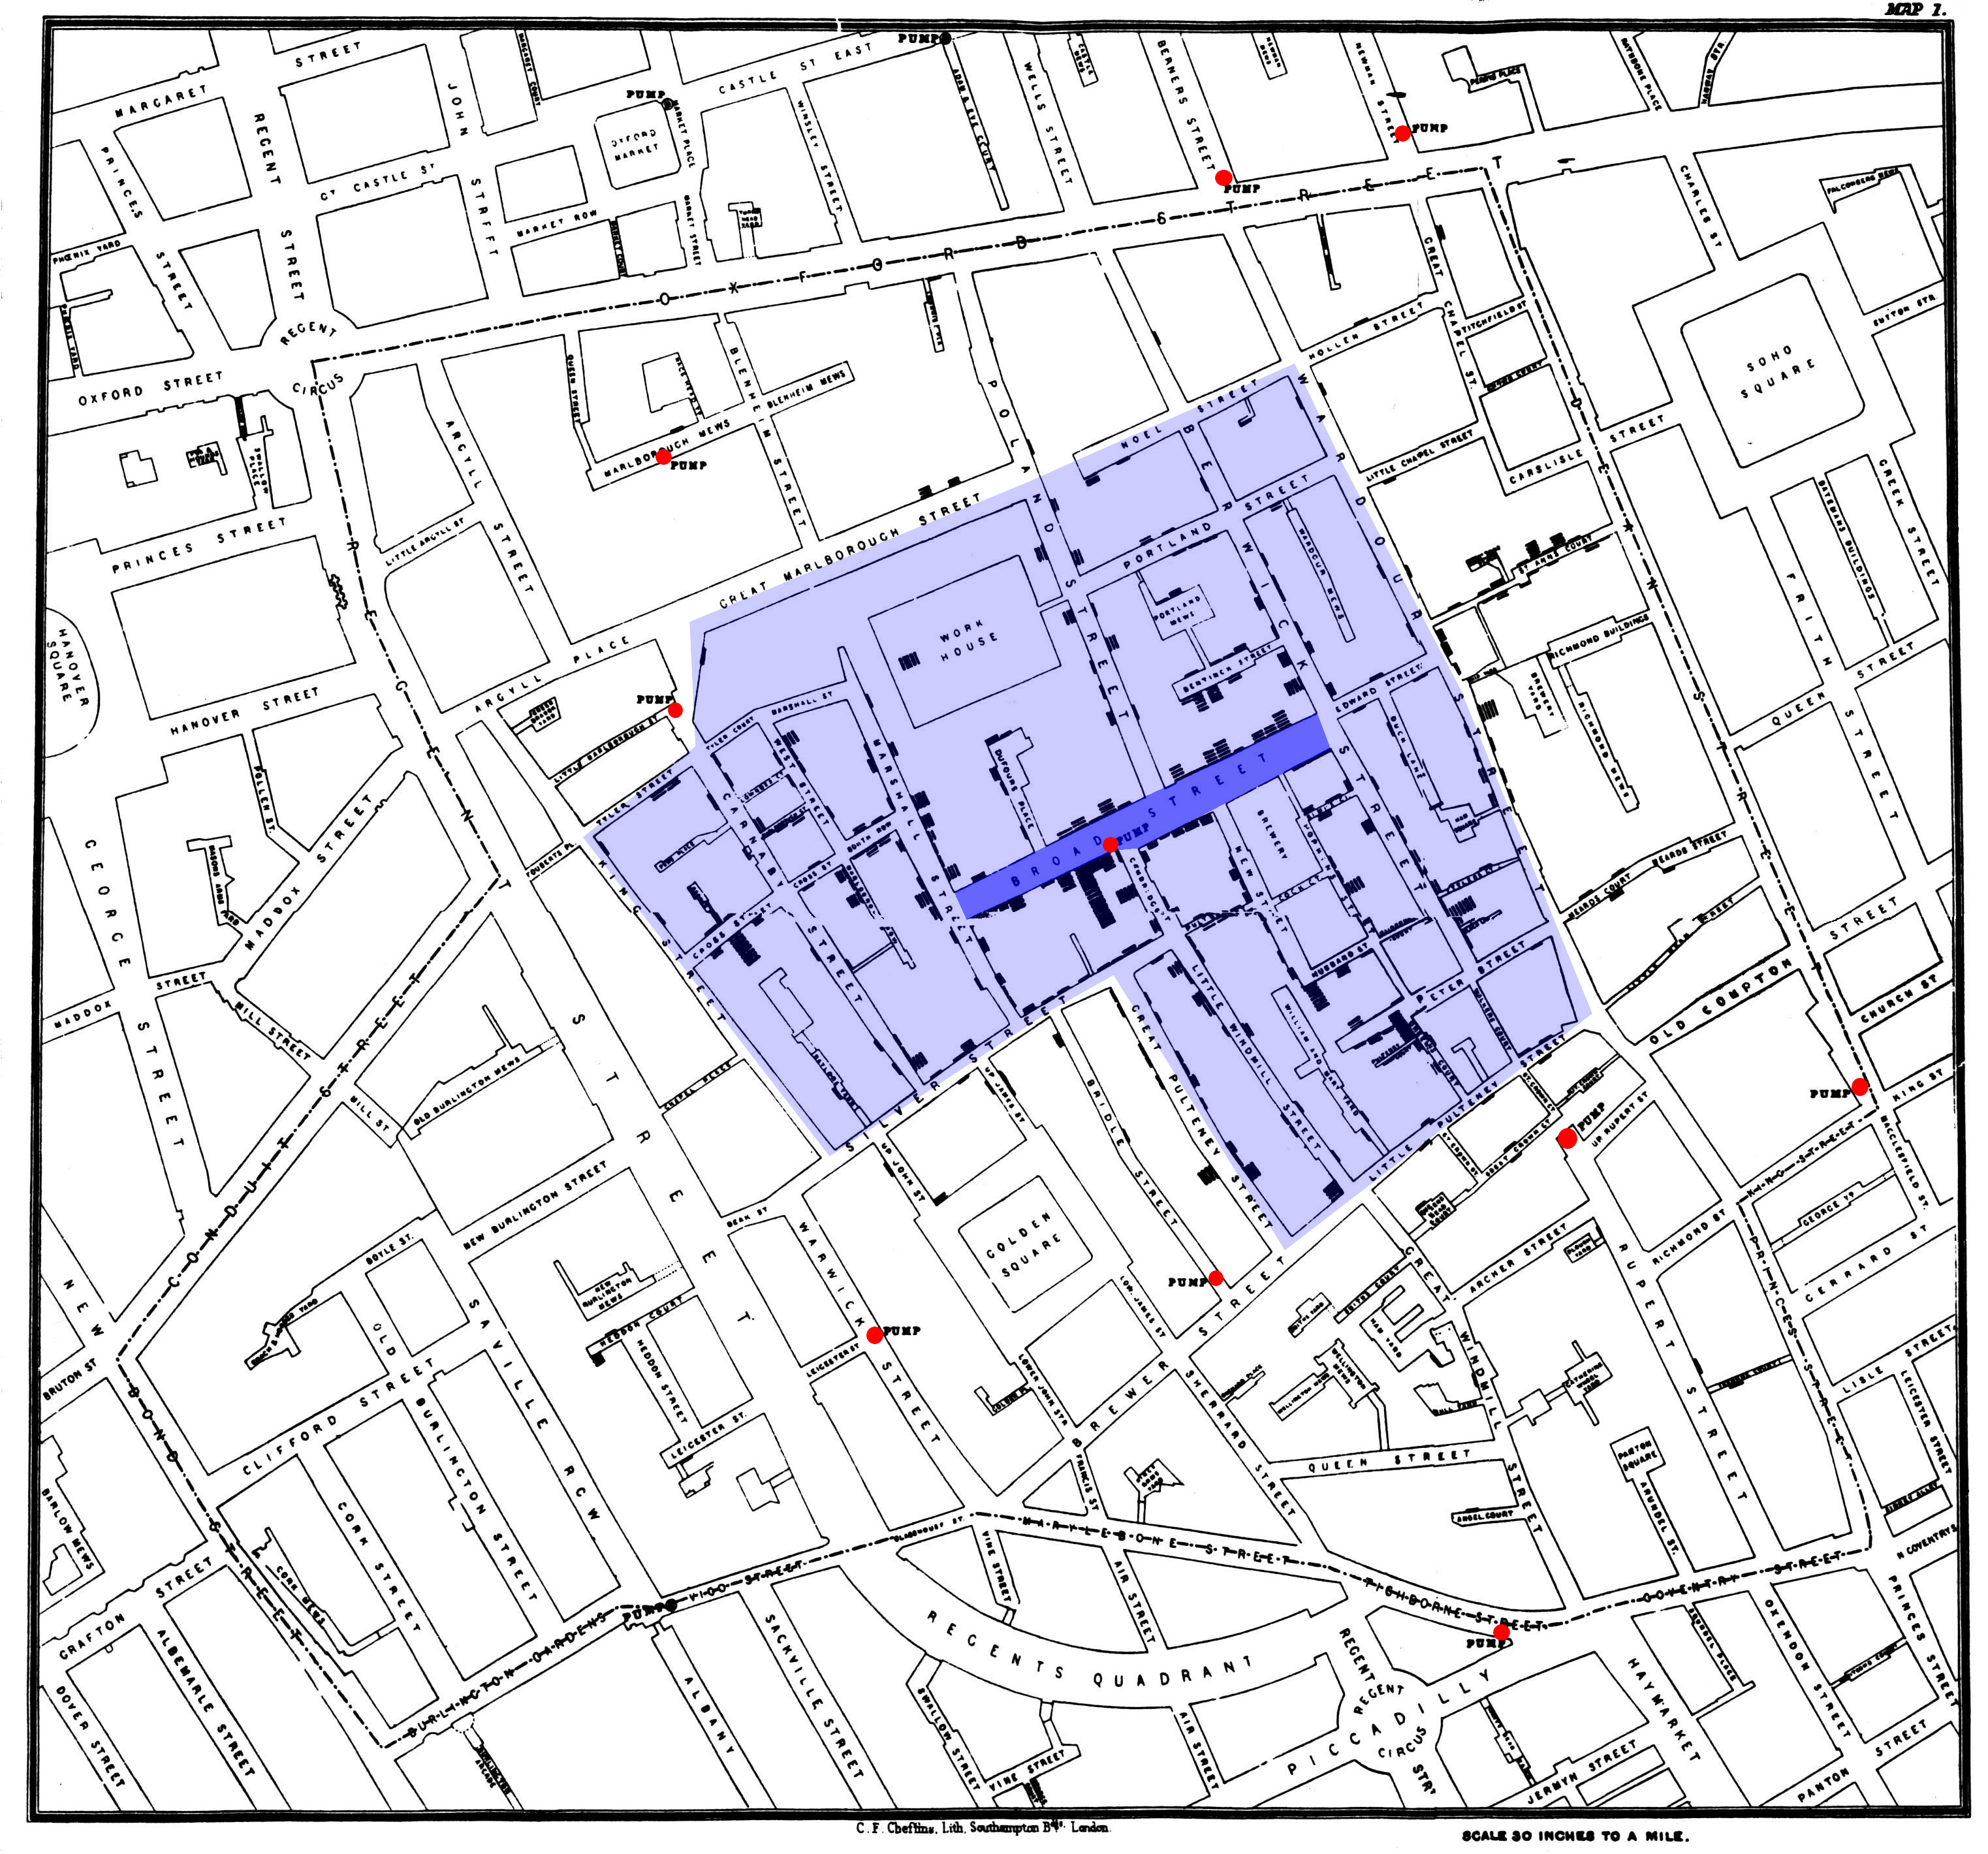
\includegraphics[height=.98\textheight]{images/broadstreet-3}}
\only<5>{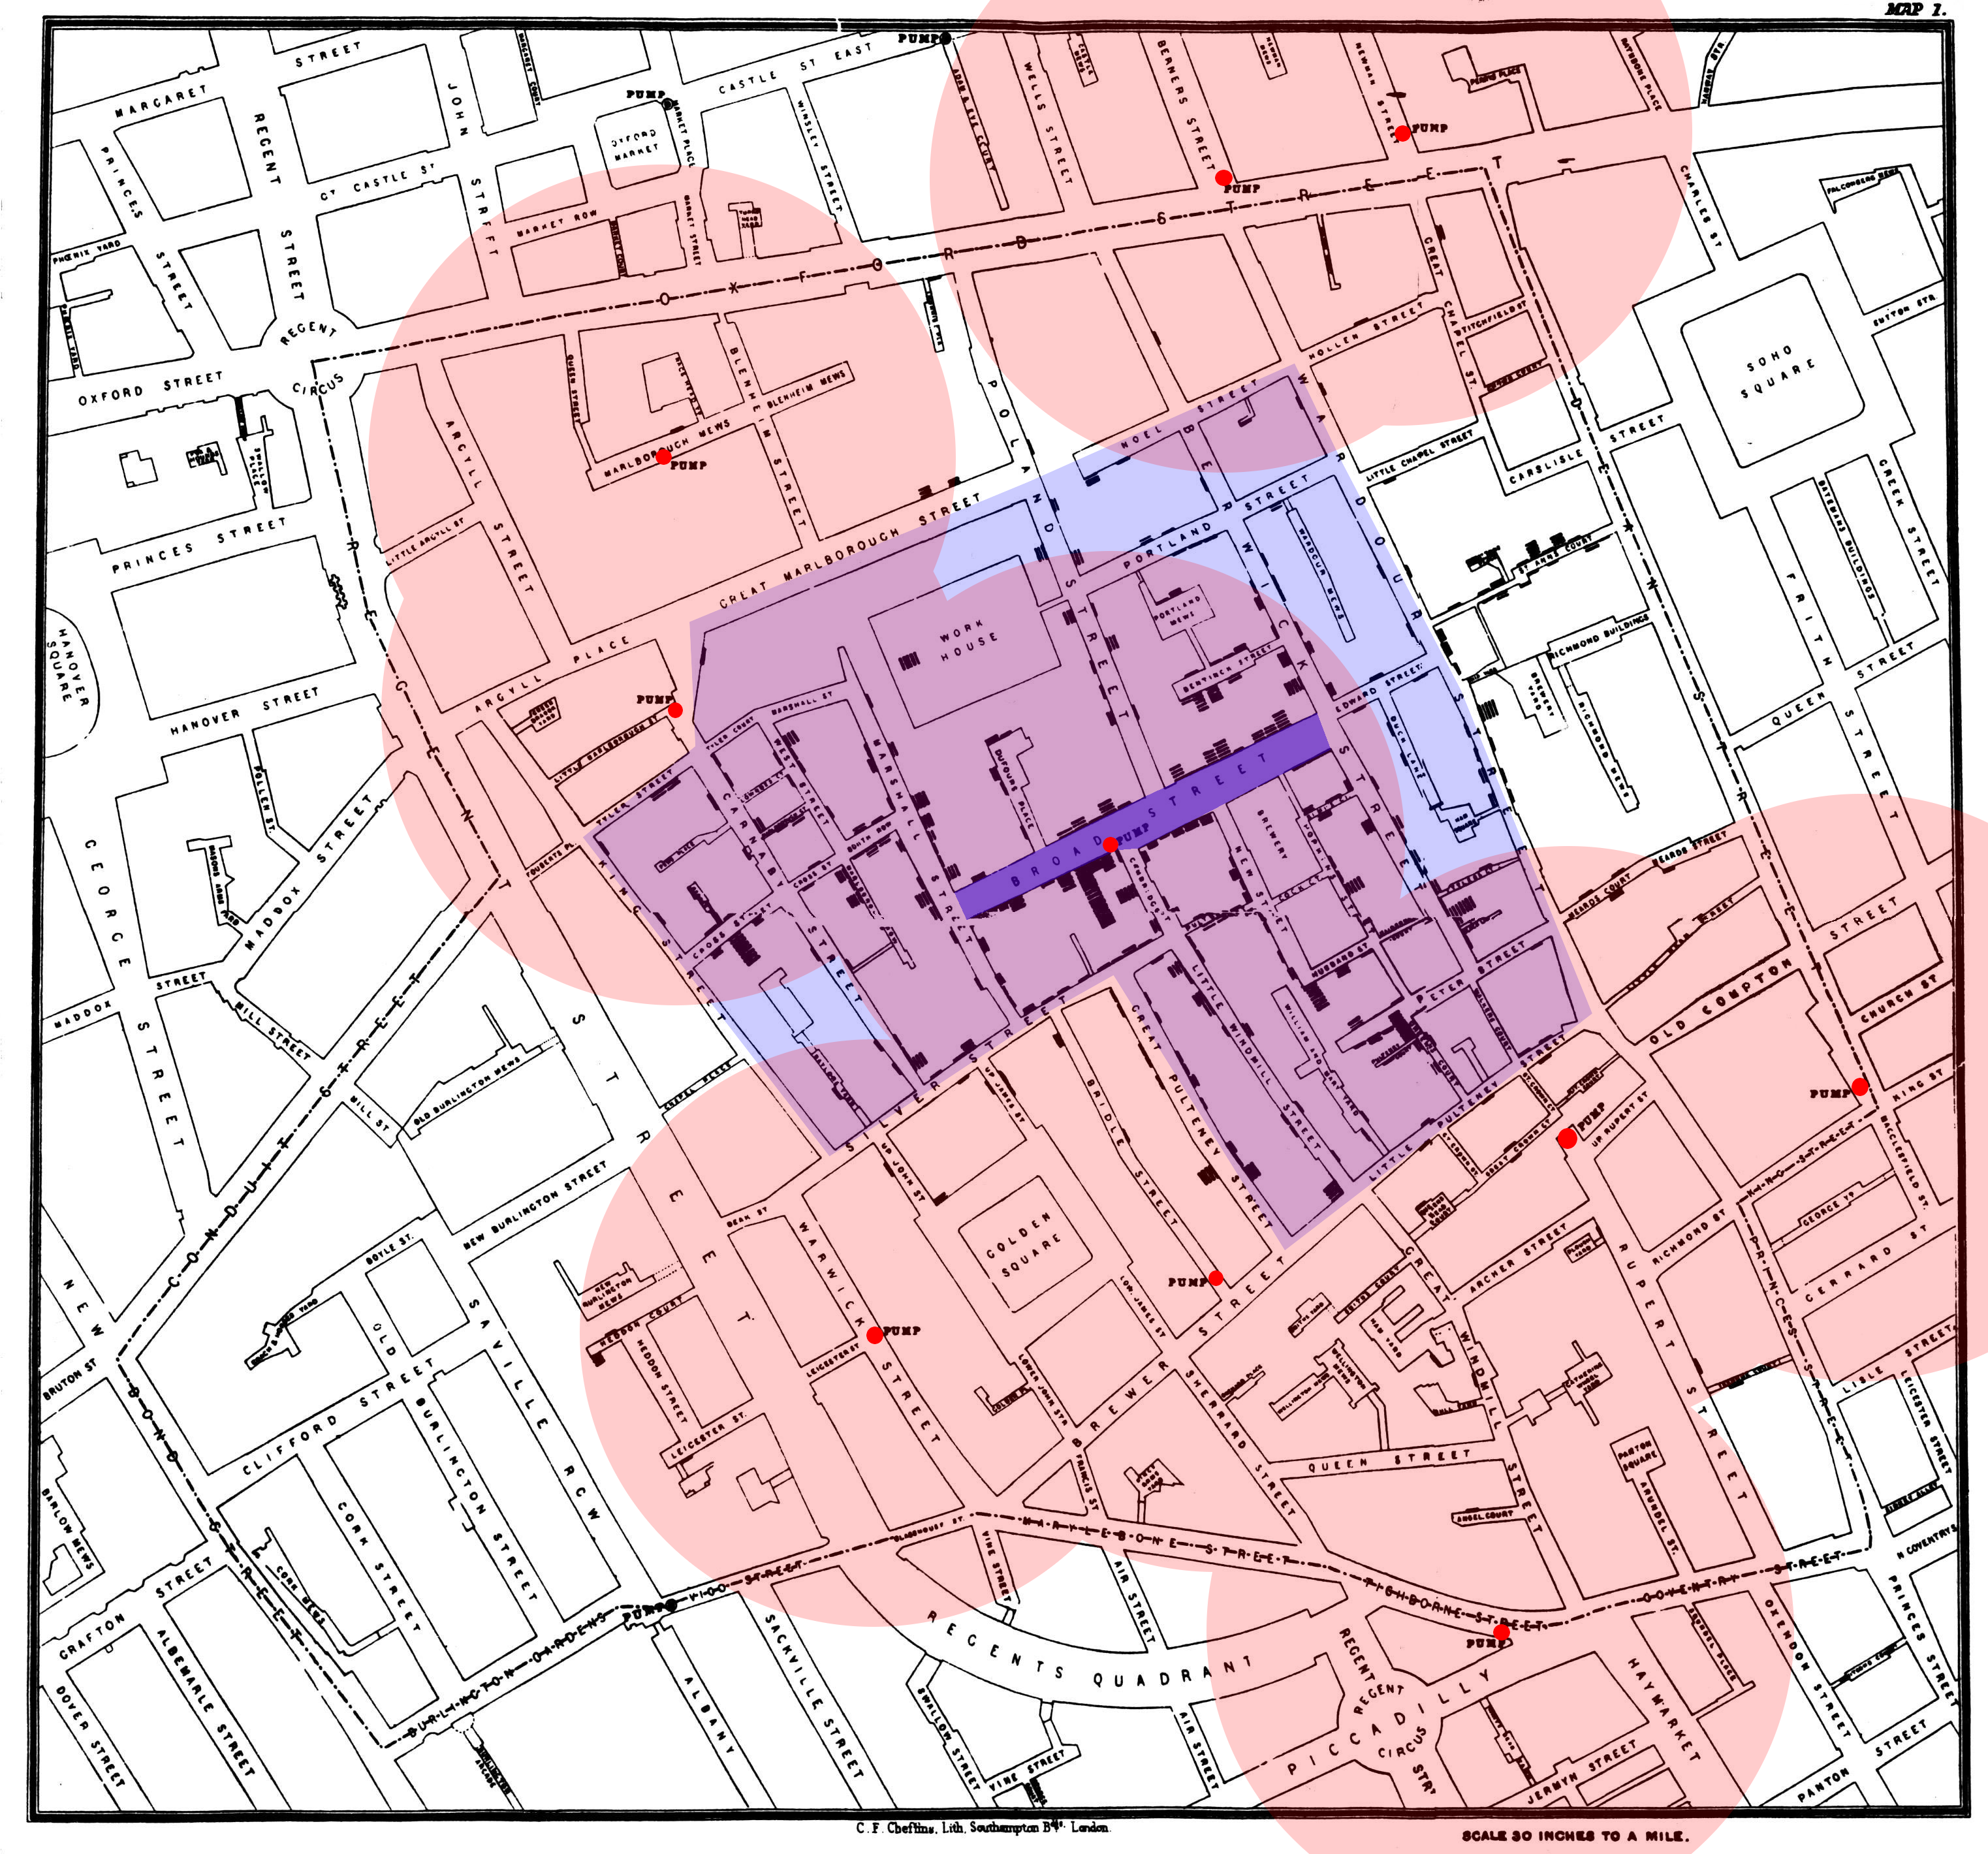
\includegraphics[height=.98\textheight]{images/broadstreet-4}}
\only<6>{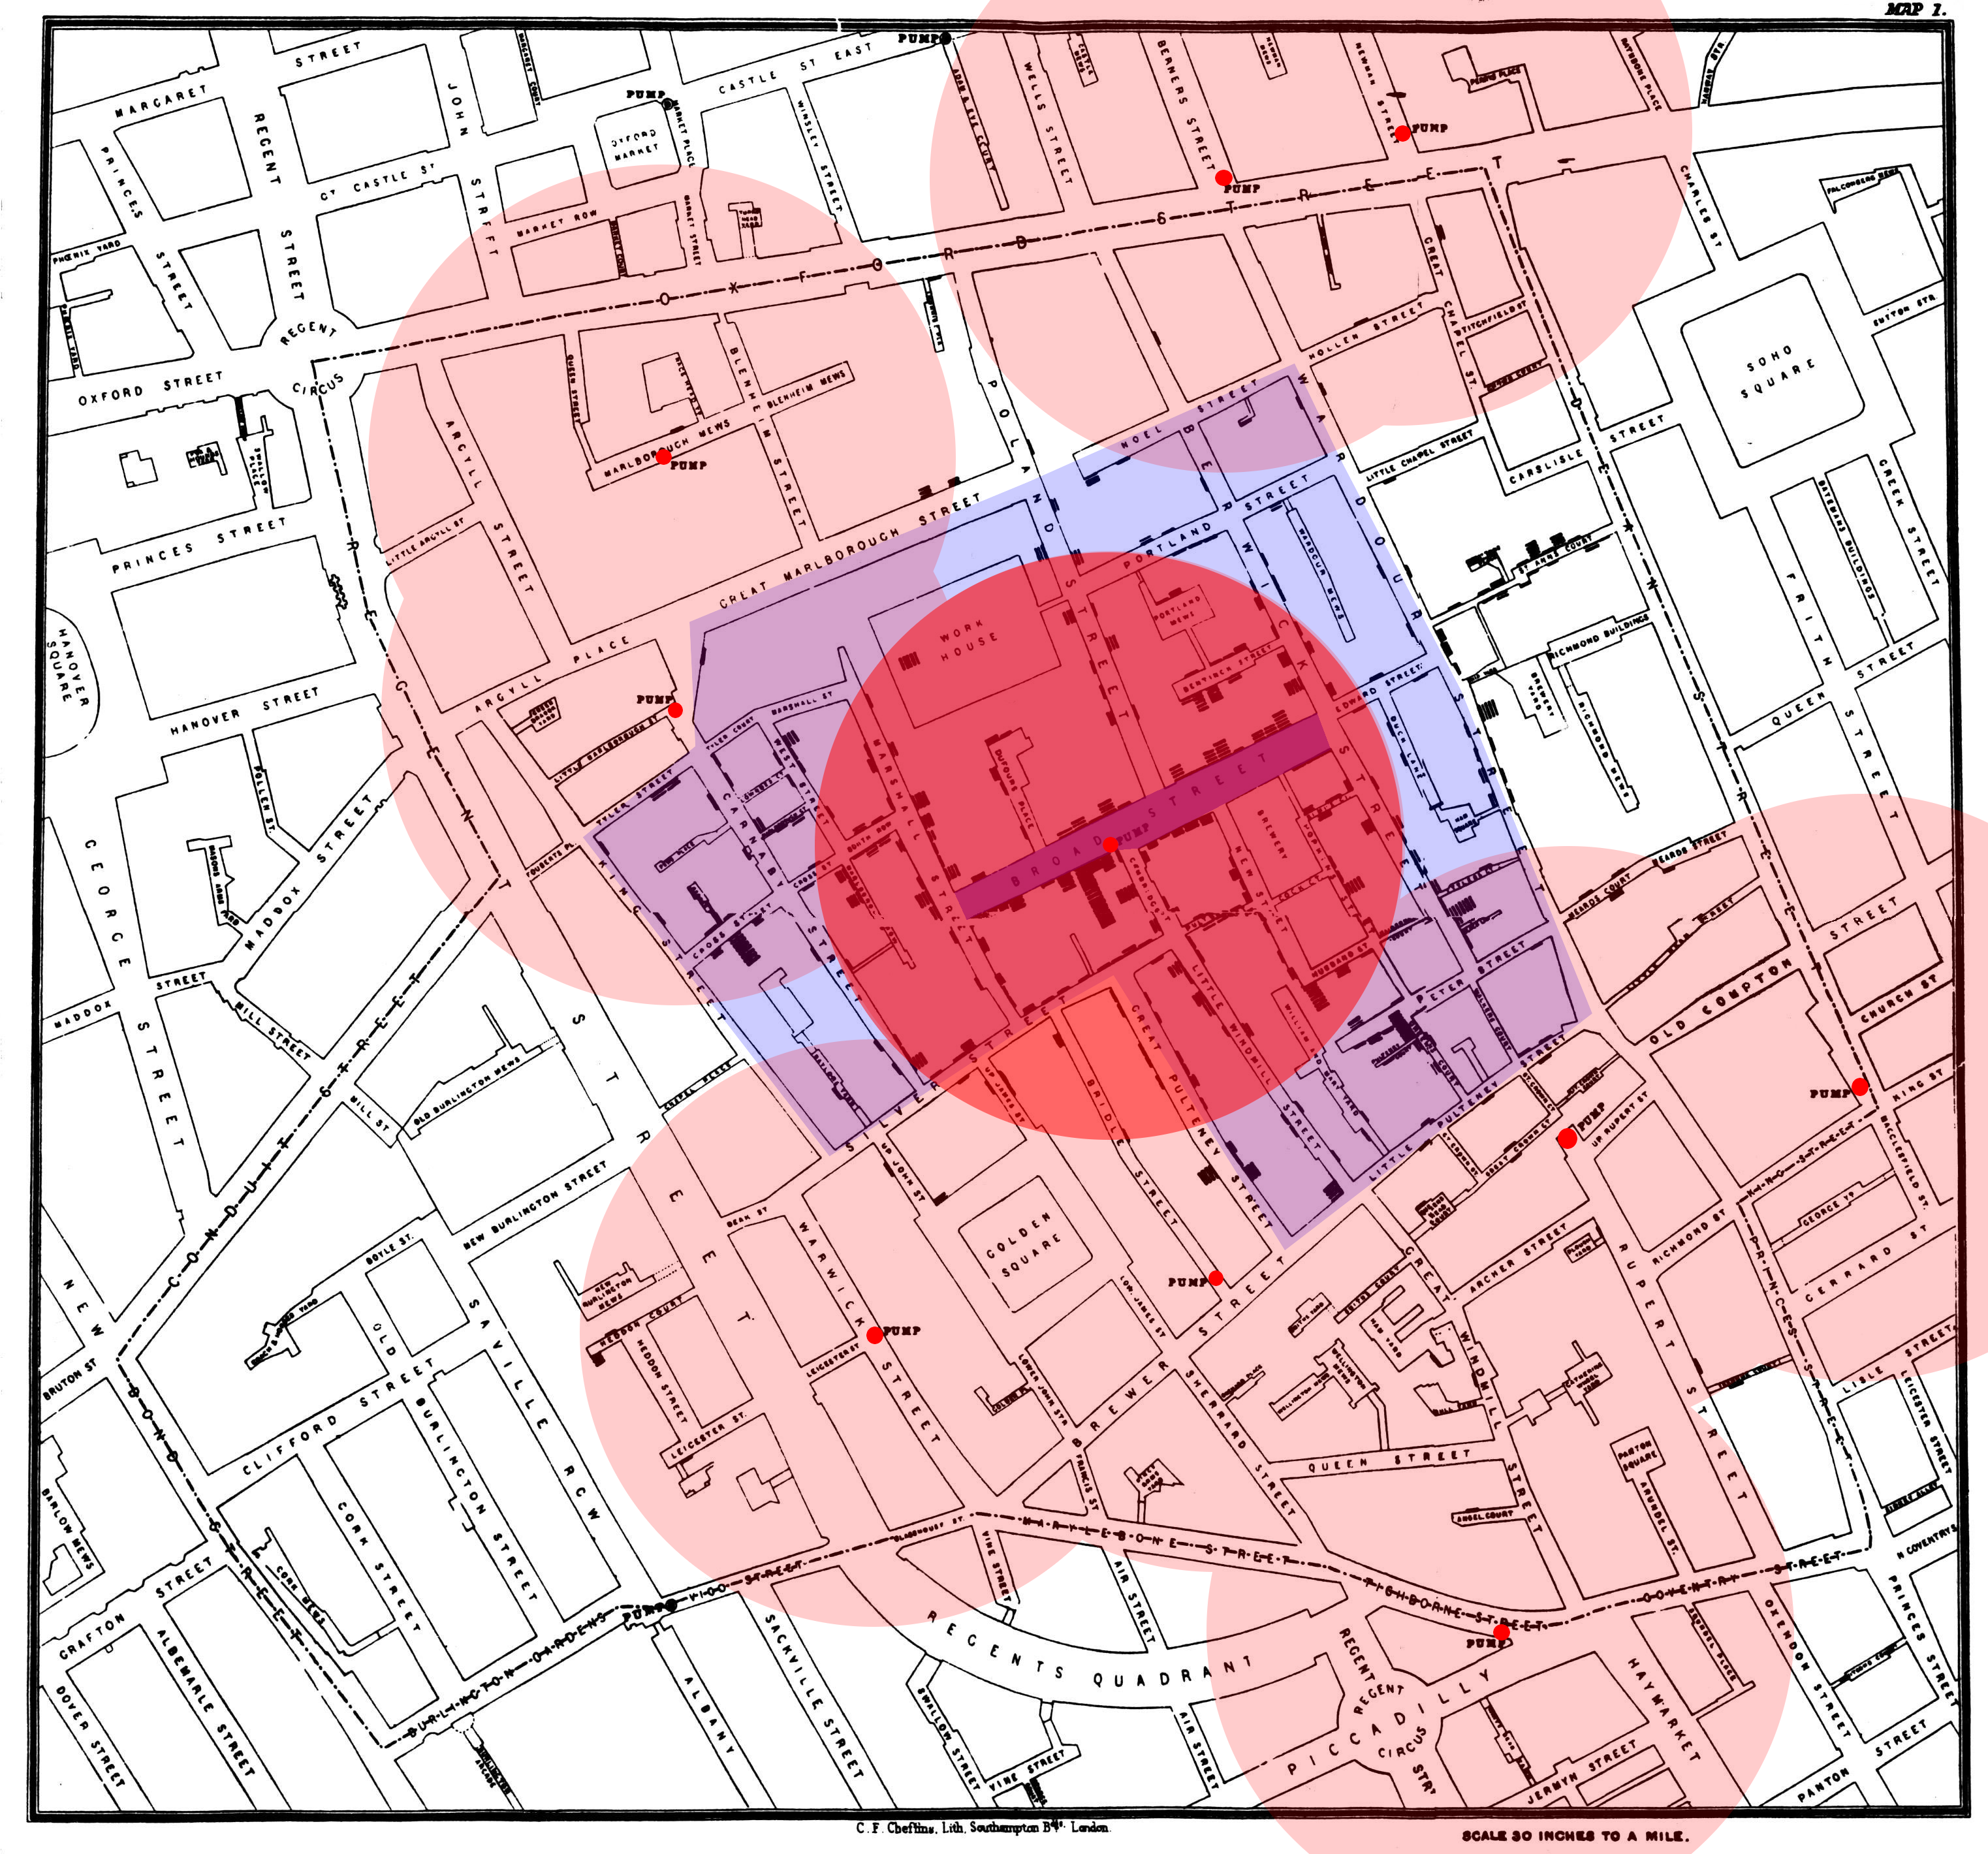
\includegraphics[height=.98\textheight]{images/broadstreet-5}}
\only<7>{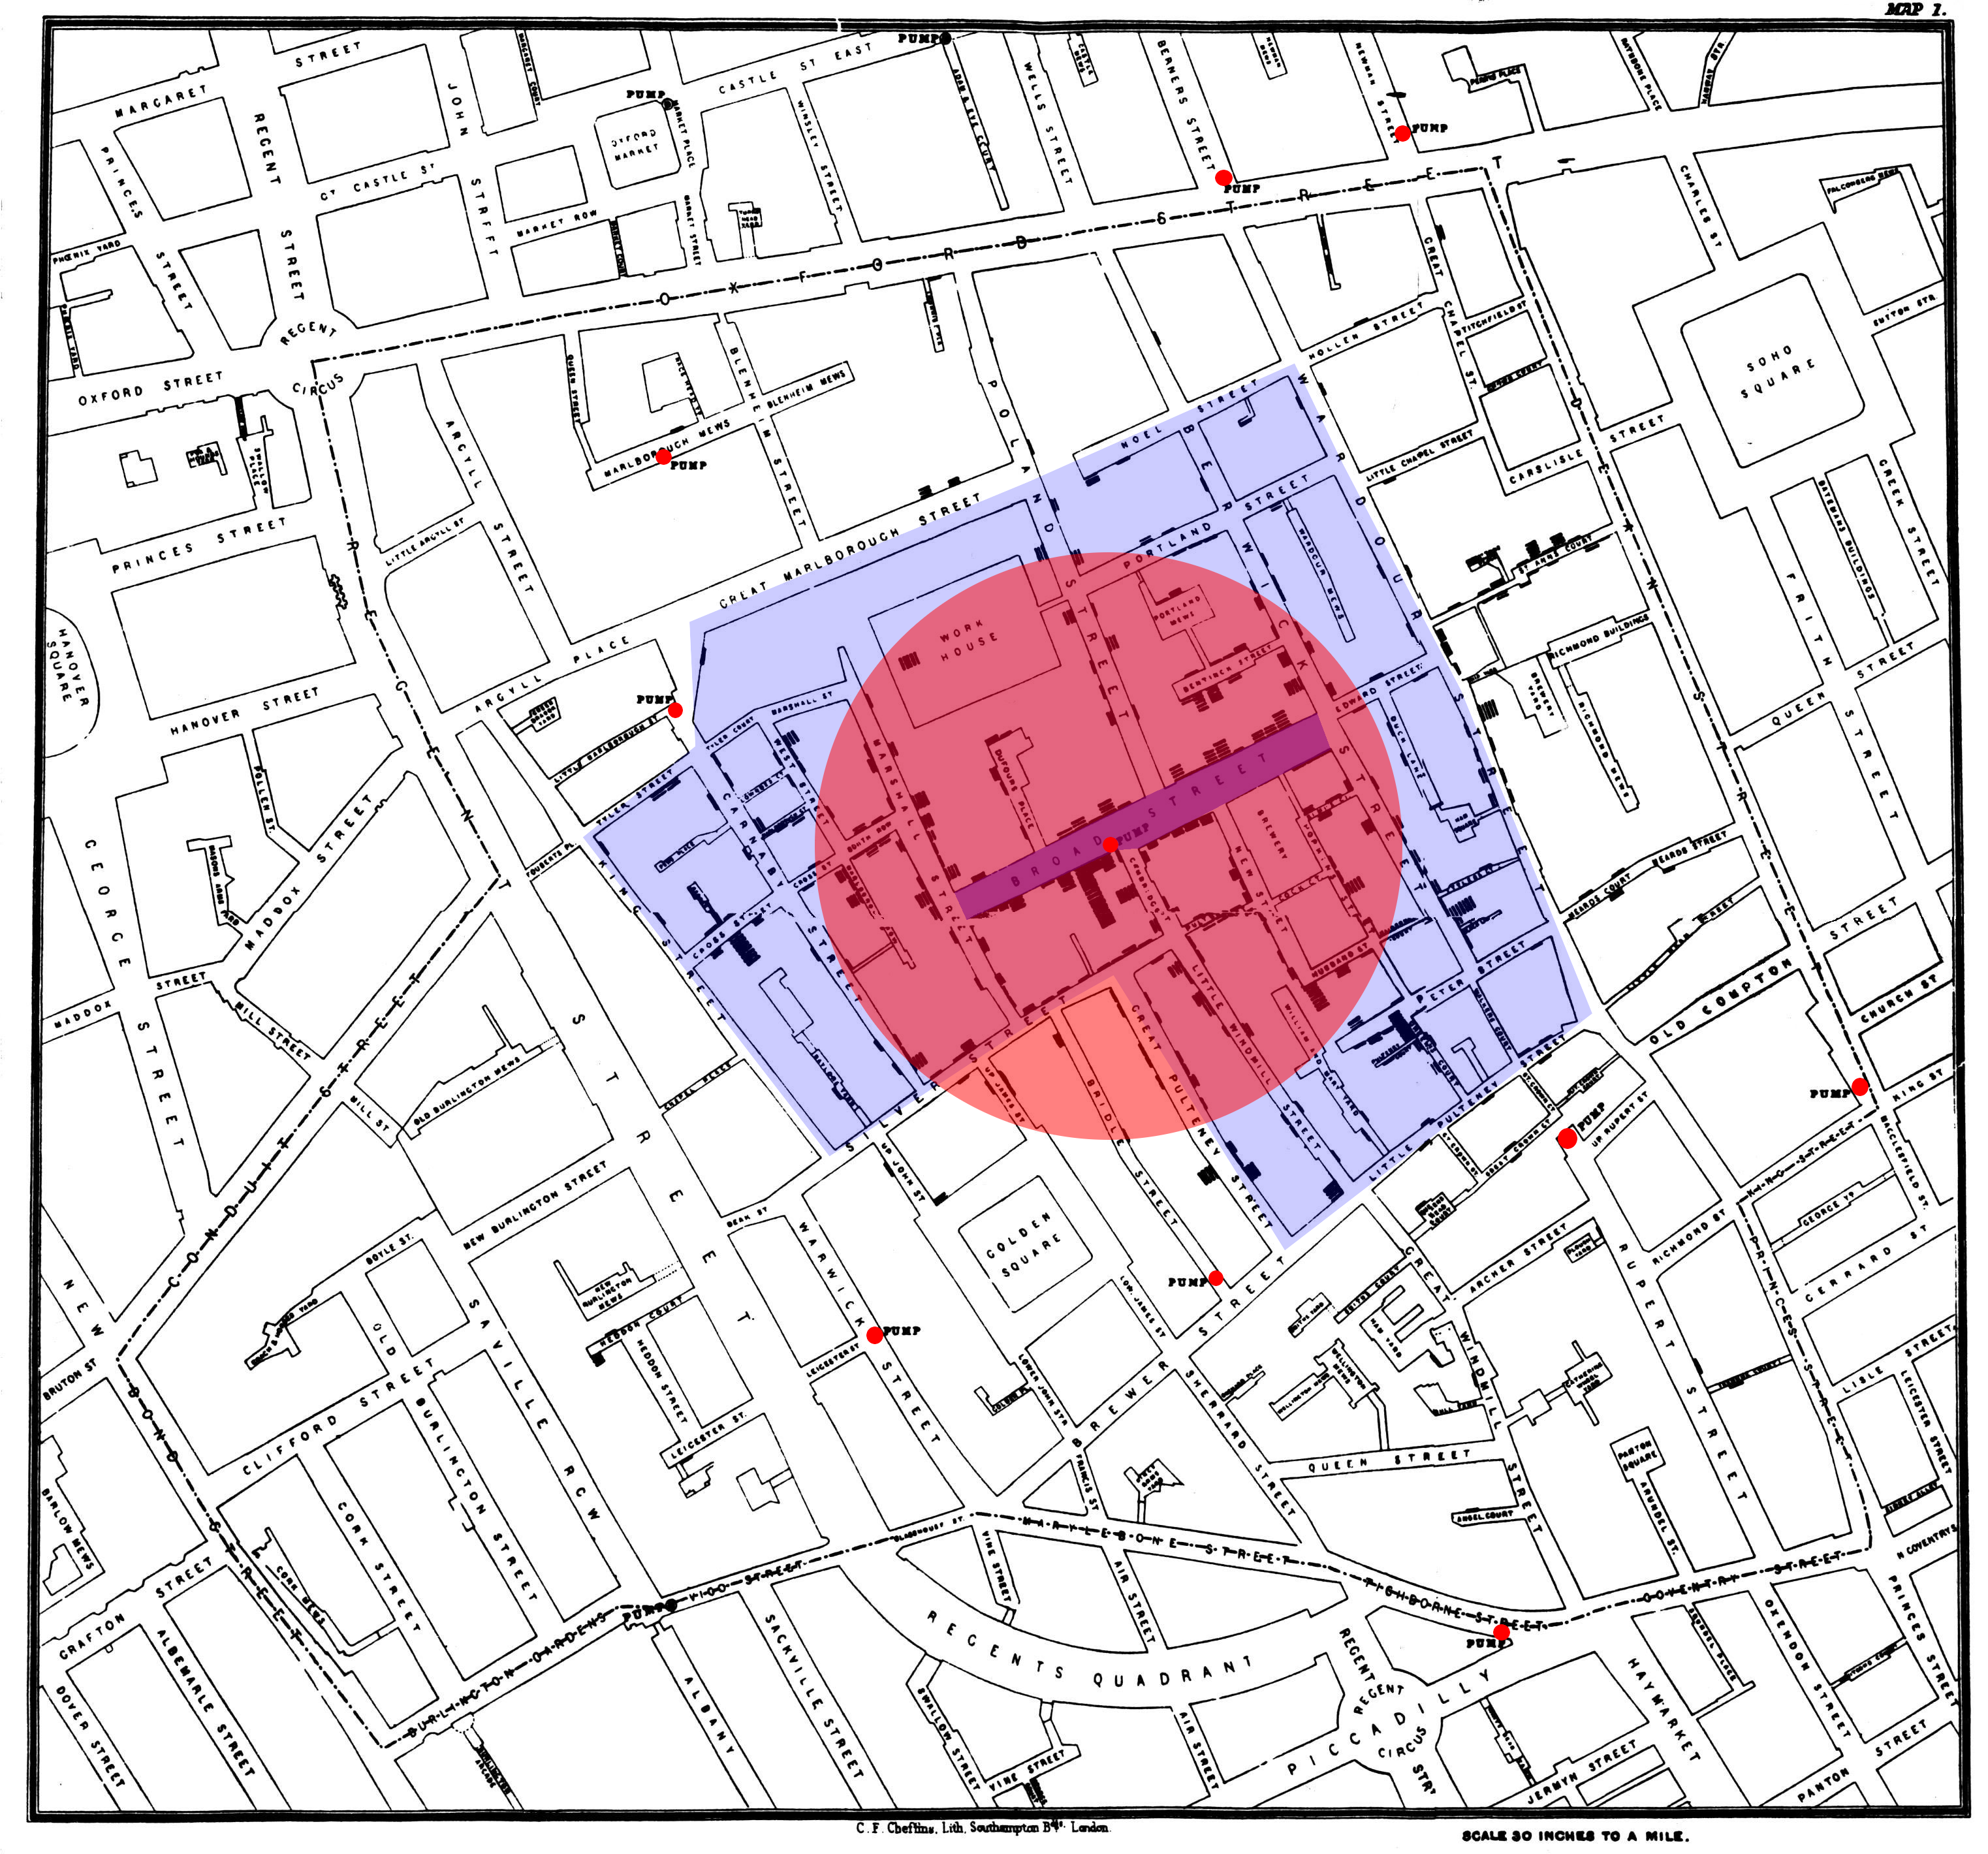
\includegraphics[height=.98\textheight]{images/broadstreet-6}}
\end{center}

{\footnotesize Image source: Public Domain from \href{https://en.wikipedia.org/wiki/File:Snow-cholera-map-1.jpg}{Wikipedia}}

}

\frame{}

\frame{
\begin{center}
\only<1>{\includegraphics[height=.98\textheight]{images/broadstreet-10}}
\only<2>{\includegraphics[height=.98\textheight]{images/broadstreet-11}}
\end{center}

{\footnotesize Image source: GPL-3 from \href{https://github.com/lindbrook/cholera}{GitHub \textit{lindbrook}}}

}


\frame{

\frametitle{{\normalsize Ex.: Gapminder Data}}

\begin{center}
\includegraphics[width=.9\textwidth]{images/gapminder}
\end{center}

}



\frame{

\frametitle{{\large \textit{Quantitative} Description}}

\begin{itemize}\itemsep0.25em
\item<2-> A \textit{rectangular}, case-by-variable dataset
	\begin{itemize}
	\item ``dataset observations'' (DSOs)
	\end{itemize}
\item<3-> A clear \textit{unit of analysis}
\item<4-> Multiple cases/units
\item<5-> Quantitative and qualitative \textit{measures}
\item<6-> Calculation of summary \textit{statistics}
\end{itemize}

}

\frame{

\frametitle{{\large Dataset Observation (DSO)}}

``\textbf<4>{a score} for \textbf<2>{a case} on \textbf<3>{a variable}''

\small 
\begin{center}
\begin{tabular}{lrrr}
State & Year & \textbf<3>{Var1} & Var2 \\
\textbf<2>{Afghanistan} & \textbf<2>{2016} & \textbf<2->{1} & \textbf<2>{TRUE} \\ 
Afghanistan & 2015 & \textbf<3>{1} & TRUE \\
Algeria & 2016 & \textbf<3>{1} & FALSE \\
Algeria & 2015 & \textbf<3>{0} & TRUE \\
\dots \\
\end{tabular}
\end{center}

}

\frame{

\frametitle{Description Beyond DSOs}

\begin{itemize}\itemsep0.5em
\item DSOs are not the only kind of data
\item Non-DSOs do not fit in a rectangular dataset
\item<2-> Sometimes hear about ``qualitative'' and ``quantitative'' research
\begin{itemize}
\item This divide is illusory because all research is qualitative and some involves quantitative data description
\end{itemize}
\item<2-> Return to this in a few weeks
\end{itemize}

}

\frame{}


% cases


\section{Measurement}
\frame{\tableofcontents[currentsection]}


\frame{
\frametitle{An Example: Opinion}

\begin{itemize}\itemsep0.5em
\item \textit{Opinion} is a summary evaluation of a particular object
\item Only one necessary feature: evaluation/favorability
\item How do we measure this?
\end{itemize}

}

% Agree/disagree
% Oppose/support
% Degree of favorability
% Warm/cool
% Positive/negative
% How many scale points?
% Implicit: text analysis, skin conductance, heart rate, implicit association test

\frame{

\frametitle{Operationalization}

\begin{enumerate}\itemsep0.5em
\item Measure features
	\begin{itemize}
	\item Level of measurement
	\item How to score each case on each feature
	\item Be concrete
	\end{itemize}
\item Aggregate feature measurements
	\begin{itemize}
	\item Sum? Average? AND logical?
	\item Level of measurement of final scale
	\item Range of possible values
	\item Justify against criticisms/alternatives
	\end{itemize}
\end{enumerate}

}

% measuring violence might require an OR logical operationalization (listing of possible forms of violence)
% might be measures of victims (number hurt or killed); this could then be interval, or reduced categorical, or binary
% might be property damage and/or victims
% attributes might need to be weighted

\frame{

\frametitle{Operationalization I}

\begin{itemize}\itemsep0.75em
\item To study concepts, we need to be able to observe those concepts and encode them as \textit{variables}
\item<2-> The definition of \textit{variable}:
	\begin{itemize}
	\item A dimension that describes an observation
	\item<3-> Or, the \textit{operationalization} of a concept
	\end{itemize}
\end{itemize}

}

\frame{

\frametitle{Some definitions!}

\begin{itemize}\itemsep1em
\item Variable: A dimension that describes an observation
\item Operationalization: the process of deciding on measures for concepts
\item Coding: Assigning a score for a variable to an observation
	\begin{itemize}
	\item<2-> Manual or hand coding
	\item<2-> Automated coding
	\end{itemize}
\end{itemize}

}



\frame{

\frametitle{Operationalization II}

\vspace{-2em}

\begin{center}
\tikzstyle{block} = [rectangle, draw, fill=blue!20!white, text width=5em, text centered, rounded corners, minimum height=1em, node distance=7em]
\begin{tikzpicture}[scale=0.5]
\draw<1-> [block] node at (0,0) (concept) {{\Large Concept}};
\draw<1-> [block] node at (-5, -3) (a1) {Attribute};
\draw<1-> [block] node at (0, -3) (a2) {Attribute};
\draw<1-> [block] node at (5, -3) (a3) {Attribute};
\draw<1-> [->, very thick] (concept) -- (a1);
\draw<1-> [->, very thick] (concept) -- (a2);
\draw<1-> [->, very thick] (concept) -- (a3);

\draw<1-> [block, align=center] node at (-11.5, -1.5) (def) {Concept Definition};
\draw<1-> [decorate,very thick, decoration={brace,amplitude=10pt},xshift=-10pt,yshift=0pt]
(-7.5,-3.4) -- (-7.5,0.5);

\draw<2-> [block] node at (-5, -8) (m1) {{\small Measure(s)}};
\draw<2-> [block] node at (0, -8) (m2) {{\small Measure(s)}};
\draw<2-> [block] node at (5, -8) (m3) {{\small Measure(s)}};

\draw<2-> [->, very thick] (a1) -- (m1);
\draw<2-> [->, very thick] (a2) -- (m2);
\draw<2-> [->, very thick] (a3) -- (m3);

\draw<2-> [block, align=center] node at (-11.5, -6.5) (def) {Operation-alization};
\draw<2-> [decorate,very thick, decoration={brace,amplitude=10pt},xshift=-10pt,yshift=0pt]
(-7.5,-8.5) -- (-7.5,-3.6);


\end{tikzpicture}
\end{center}


}

\frame{

\frametitle{Operationalization III}

{\Large

Definition\\ 
	\onslide<2->{\hspace{1em} $\rightarrow$ Feature} \\
	\onslide<3->{\hspace{3em} $\rightarrow$ Indicator(s)}
}

\vspace{1em}

\onslide<4-5>{Indicators might be scaled or potential alternatives}
}


% think about cases: given your measures of ``free and fair elections'', how does Britain score on each of those?


\frame{

\frametitle{Example: Democracy}

{\Large

Democracy\\ 
	\onslide<2->{\hspace{1em} $\rightarrow$ Free and fair elections} \\
	\onslide<3->{\hspace{3em} $\rightarrow$ ?}
}

\vspace{1em}
How do we operationalize this concept?
}





\frame{\huge\vskip20pt\textbf{Questions?}}


\frame{

Once we have an operationalization, \textit{coding} turns observations of attributes into DSOs

\begin{center}
\begin{tabular}{lccc}
Case & Measure1 & Measure2 & Measure3 \\ \hline
UK & ? & ? & ? \\
France & ? & ? & ? \\
Germany & ? & ? & ? \\
Spain & ? & ? & ? \\
\dots \\ \hline
\end{tabular}
\end{center}


}


\frame{

\frametitle{Types of Measures}

\begin{braceitems}\itemsep1em
\item \nt{Categorical}
	\begin{itemize}
	\item Binary
	\end{itemize}
\item \nt{Ordinal}
\item \nt{Interval}
\end{braceitems}
\makebrace{1}{2}{Qualitative}
\makebrace{2}{3}{Quantitative}

\vspace{0.5em}

{\footnotesize Note: \textit{Ratio} scale measures are interval measures with a non-arbitrary zero value}

}

% describe difference between qualitative and quantitative
% qualitative is assigning a descriptive label
% quantitative is assigning a numerical value

% describe the three types


\frame{

\frametitle{Activity}

\begin{itemize}\itemsep0.5em
\item Concept: Democracy
\item Attribute: Free and fair elections
\item Measure:
	\begin{enumerate}
	\item Categorical
	\item Ordinal
	\item Numeric
	\end{enumerate}
\end{itemize}

}


\frame{

\frametitle{Why do we care?}

\begin{center}

Once we have measured \textit{variables} for \textit{observations}, we can conduct \textit{analysis}!

\vspace{1em}

\only<2>{And once we have analysis, we can \textit{draw inferences} and \textit{make evidence-based claims}.}

\end{center}

}



\frame{\huge\vskip20pt\textbf{Questions?}}



\section{Assessing Measurement Quality}
\frame{\tableofcontents[currentsection]}

\frame{

\frametitle{{\large Assessing Measurement Quality}}

\begin{enumerate}\itemsep1em
\item Conceptual clarity
\item Construct validity
	\begin{itemize}
	\item Convergent validity
	\item Divergent validity
	\end{itemize}
\item Accuracy and precision
\end{enumerate}

}

\frame{
\frametitle{Assessing Measures I}

\begin{itemize}\itemsep1em
\item \textit{Conceptual clarity} is about knowing what we want to measure
\item Sloppy concepts make for bad measures
	\begin{itemize}
	\item Ambiguity % multiple meanings or multiple labels
	\item Vagueness % concept without a definition
	\end{itemize}
\item<2-> Revise concept definition as needed
\end{itemize}
}


\frame{
\frametitle{Assessing Measures II}

\begin{itemize}\itemsep0.5em
\item \textit{Construct validity} is the degree to which a variable measures a concept
\item<2-> Construct validity is \textbf{high} if a variable is a measure of the concept we care about
\item<3-> Construct validity is \textbf{low} if a variable is actually a measure of something else
\end{itemize}
}

% sources: bad concept definition; totally inappropriate measures (using income to measure weight); measure becomes the concept (actual income is replaced by self-reported income)


\frame{
\frametitle{Example: Polity IV\footnote{http://www3.nd.edu/~mcoppedg/crd/PolityIVUsersManualv2002.pdf}}

\footnotesize

Institutionalized Democracy: \textit<2->{Democracy is conceived as three essential, interdependent elements}. One is the \textbf<3->{presence of institutions and procedures through which citizens can express effective preferences about alternative policies and leaders}. Second is the existence of \textbf<4->{institutionalized constraints on the exercise of power by the executive}. Third is the \textbf<5->{guarantee of civil liberties to all citizens in their daily lives and in acts of political participation}. Other aspects of plural democracy, such as the rule of law, systems of checks and balances, freedom of the press, and so on are means to, or specific manifestations of, these general principles. We do not include coded data on civil liberties.

}

\frame{
\centering
\includegraphics[height=.9\textheight]{images/polity}
}


\frame{

\frametitle{{\large Assessing Construct Validity}}

\begin{itemize}\itemsep1em
\item Multiple measures!
\item Look for:
	\begin{itemize}
	\item Convergence (Convergent validity)
	\item Discrimination (Discriminant validity)
	\end{itemize}
\item<2-> For example, the multi-trait, multi-method matrix
\end{itemize}
}

% two (or more) measures of the same concept are highly correlated; scaling
% two (or more) measures of distinct concepts are not correlated
% Measures of distinct concepts may be correlated if they are causally related to one another, so simple correlations do not mean two measures are necessarily of the same concept

% mention predictive validity (what Kellstedt and Whitten call construct validity)


\frame{

\frametitle{{\large Using Multiple Indicators}}

\begin{itemize}\itemsep1em

\item Choose the ``best'' one

\item Apply an AND operator
	\begin{itemize}
	\item Must have all indicators to be coded 1
	\item Treat indicators as ``ordinal'' in Gerring's sense
	\end{itemize}

\item Scale the indicators (e.g., sum or mean)

\end{itemize}

}

% do you add? do you average? do you count some indicators more than others?




\frame<1-2>[label=challenges3]{

\frametitle{Assessing Measures III}

\Large

\begin{itemize}\itemsep1em
\item<2-> Accuracy
\item<3-> Precision
\item<4-> Reliability
\end{itemize}

}

\frame{
\frametitle{Accurate}
{\small Synonyms: true, correct, unbiased, valid}\\
\vspace{1em}

\includegraphics[width=\textwidth]{images/kilogram}

{\tiny \href{https://commons.wikimedia.org/wiki/File:MassStandards_005.jpg}{Image Source: Wikimedia}, Public Domain}
}

\againframe<2-3>{challenges3}


\frame{
\frametitle{Precise}
{\small Synonyms: certain, exact, specific, low variance}\\

\begin{center}
\includegraphics[width=0.6\textwidth]{images/accuracyprecision}
\end{center}

\vspace{-1em}
{\tiny \href{https://commons.wikimedia.org/wiki/File:Reliability_and_validity.svg}{Image Source: Wikimedia}, Nevit Dilmen}
}


\againframe<3-4>{challenges3}


\frame{
\frametitle{Reliable}
{\small Synonyms: dependable, replicable, repeatable, consistent}\\

\vspace{1em}

Typically used in the context of:

\begin{itemize}
\item Multiple measures used in a scale % scale reliability
\item Multiple scores at different times % test-retest reliability 
\item Multiple individuals coding using one method % inter-coder/inter-rater reliability
\end{itemize}

}

% Multiple measures


\frame{\huge\vskip20pt\textbf{Questions?}}


\frame{
\frametitle{Key Points}

\begin{enumerate}\itemsep1em
\item We want to make claims about \textit{concepts}
\item But we only observe and can only analyse observed, measured \textit{variables}
\item So our task as scientists is to:
	\begin{itemize}
	\item Link the concepts we care about to observable phenomena
	\item Draw out theoretical implications from measures
	\end{itemize}
\end{enumerate}
}



\appendix
\frame{}

\end{document}
